\documentclass{beamer}

\usepackage[utf8]{inputenc}
\usepackage[T1]{fontenc}
\usepackage[croatian]{babel}

\title{Detekcija pješaka u urbanim okruženjima korišenjem značajki temeljenih na teksturi i boji}
\author{Iva Miholić, Gustav Matula, Kristijan Franković, Tomislav Kiš}

\begin{document}
\begin{frame}
\maketitle
\end{frame}

\begin{frame}
\frametitle{Detekcija pješaka u urbanim okruženjima}
\framesubtitle{Opis zadatka i postojećih rješenja}
\begin{itemize}
\item detekcija objekta u okviru područja računalnog vida
\item detektor pješaka na fotografijama iz urbanih okruženja korištenjem značajki temeljenih na teksturi i boji.
\end{itemize}
\end{frame}

\begin{frame}
\begin{itemize}
\item primjena \emph{VJ} detektora objekata
\item detektori temeljeni na histogramu usmjerenih gradijenata \emph{Histogram of Oriented Gradients, HOG}
\item HOG uz linearni SVM u kombinaciji sa drugim značajkama temeljenih na svojstvima boje, tekstura i oblika
\item složeniji postupci ne daju bolje rezultate
\end{itemize}
\end{frame}

\begin{frame}
\begin{itemize}
\item metoda skalabilnog kliznog prozora
\item ignoriranje konteksta oko okvira koji se promatra 
\end{itemize}
\begin{figure}
\center
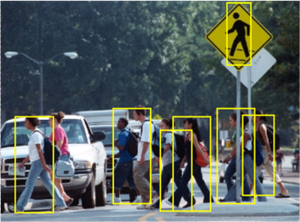
\includegraphics[scale=0.7]{img/crossing.png}
\caption{Fotografija koja je klasificirana detektorom pješaka metodom kliznog prozora. Žuti okviri prikazuju okvire onih prozora koji su klasificirani kao prikaz pješaka.}
\label{primjer_klasifikacije}
\end{figure}
\end{frame}

\begin{frame}
\frametitle{Prostor značajki}
\begin{itemize}
\item najviše korištene značajke temeljene na informaciji o bridovima, boji, teksturi lokalnim oblicima te svojstvima gradijenta i kovarijance
\item proširenje prostora značajki može biti problematično za klasične algoritme učenja 
\item redukcija prostora značajki metodom Fisherove diskriminantne analize ili postupkom parcijalnih najmanjih kvadrata \emph{Partial Least Squares, PLS}
\end{itemize}
\end{frame}

\begin{frame}
\frametitle{Baza podataka za treniranje i verifikaciju rješenja}
\end{frame}

\begin{frame}
\frametitle{Idejno rješenje i prikaz arhitekture sustava računalnog vida}
\framesubtitle{Pregled značajki temeljenih na teksturi i boji}
\end{frame}

\begin{frame}
\framesubtitle{Plan arhitekture sustava računalnog vida}
\end{frame}
\end{document}